\section{Data driven business models}
\label{s:DDBM}
\subsection{Introduction}

% What are DDBMs? Situate them, the difference with other business models.

Companies provide value to their customers by employing a \gls{BM}, which is a relevant but not standardized topic. Due to the competitive nature of current markets, \gls{BM}s are used to maintain an advantage over competitors \cite{Hunke2017}. They are utilized to evaluate business strategies, prepare for future changes, and develop a strategy to stand out in the market.
A. Sorescu \cite{Sorescu2017} proposes three main attributes: 

\begin{itemize}
    \item Value creation
    \item Value delivery
    \item Value appropriation
\end{itemize}

Value creation covers the development process of the services or products the company offers. This can be done through providing a unique product or enhancing the efficiency of existing ones. 
In the case of value delivery, the focus lies on the products and the environment itself. How can the customer interact with the offered product or service?
Finally, value appropriation takes the financial situation into account. The purpose of this attribute is to evaluate the offered values and adapt to customer's needs. 

Another way to look at \gls{BM}s is described by the following attributes \cite{Zott2011}:

\begin{itemize}
    \item Participants
    \item Relationship between partners and customers
    \item Flow of products 
\end{itemize}

Clearly, this view is more socially driven in comparison to the first proposal. The focus does not only lie on the offered value, but also takes the fluency of value exchanges in to account.  
A \gls{BM} adapts according to the needs of the company, the competitors, and the customers. 
Although there are a wide range of \gls{BM}s, our focus lies on the \gls{DD} approach because of the relevancy with the aforementioned methods. The value creation in these models is firmly correlated to the personal data of their target group \cite{Zott2011}.

\subsection{Types of data-driven business models}

% Introduction: No agreement, different models
% Leaning towards services 
% All heavily reliant on data.

Up to this point, there is no agreement on the representation and classification of \gls{DDBM}s. 
Although different models exist and function wonderful in their specific environment, all of them need to define four main attributes, as depicted in Figure \ref{fig:DDBM overview} \cite{Hartmann2016}.

\subsubsection{Value offered}
\label{s:value offered}
Categorizing the models according to the value they offer proves to be a fitting first breakdown. 

\begin{itemize}
    \item Product
    \begin{itemize}
        \item Raw Data
        \item Applications
    \end{itemize}
    \item Service
    \begin{itemize}
        \item Information
        \item Insights
    \end{itemize}    
\end{itemize}

Service-based models can be distinguished from product-based models. 
The former is responsible for the creation of an environment or platform that offers benefits to their target group, while product-based models provide usable products \cite{Zolnowski, Visnjic2016}. 
Businesses with a focus on big data opt to utilize a service-based model, although offering raw data or applications is a common practise. 
The reason for the high demand of raw data is explained by the fact unprocessed personal data contains more detailed information which can be used more efficiently.
This however violates the expected privacy principals.
The value lies in the fact that an enormous amount of knowledge can be gained from analysing and distributing personal data. This information offers feedback as value and attempts to provide useful insights. 

\begin{figure*}[t]
\centering
    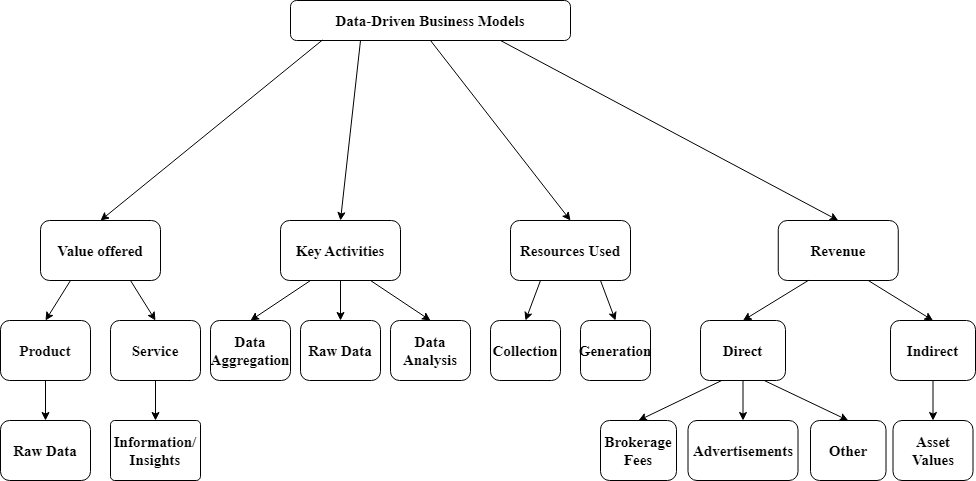
\includegraphics[width=\textwidth]{figures/ddbm.png}
\caption{A structured view on different aspects of \gls{DDBM}s \cite{Hartmann2016}}
\label{fig:DDBM overview}
\end{figure*}

\subsubsection{Resources used}

Since data is the main component in constructing a \gls{DDBM}, the chosen strategy to obtain the required data is the foundation of the model.
Hence, the reason for offering raw data in the first place.

\begin{itemize}
    \item Collection
    \begin{itemize}
        \item Web Crawlers \cite{web_crawler}
    \end{itemize}
    \item Generation
    \begin{itemize}
        \item Crowdsourcing \cite{Brabham2008}
    \end{itemize}
    
\end{itemize}

As mentioned in Section \ref{s:DataCollectionGeneration}, data can be acquired through collection or generation of data. 
Even though utilizing exclusively available data is certainly a valid strategy, some companies obtain their data directly from customers or partners. 
Combining both ways results in models that heavily rely on data acquired from social media.
This is of great importance for the subject of this paper, since Big Tech companies are focused on acquiring personal data through similar means.
Lastly, current companies resort to crowdsourcing or web crawlers \cite{Hartmann2016, web_crawler, Brabham2008}.

\subsubsection{Key activities}

The fundamental distinctions of \gls{DDBM}s are prominent in their key activities. 

\begin{itemize}
    \item Data Aggregation
    \item Data Analysis
    \item Raw Data
    \item Processing
\end{itemize}

The first approach is data aggregation, consisting of summarizing data from various sources, processing it subsequently, and finally providing a comprehensible presentation \cite{data_aggregation}.
Another crucial approach for different \gls{BM}s is data analysis. By performing a data analysis, a significant part of the work load reduces and simplifies the further process.
Because there is a need to fuel the data aggregation and analysis models with data, other models focus on data generation, providing more or specific data for their partners or customers. 
In some cases, the customer prefers already processed data. 

\subsubsection{Revenue}

Seeing that the values contribute to a sizeable part
of the model, it also has to feature a defined way to
generate revenue in exchange for the offered services.

\begin{itemize}
    \item Direct
    \begin{itemize}
        \item Brokerage Fees
        \item Advertisements
        \item Other
    \end{itemize}
    \item Indirect 
    \begin{itemize}
        \item Asset Values
    \end{itemize} 
\end{itemize}

On the one hand, \gls{BM}s could focus on direct revenue, which refers to an instantaneous gain of income.
Brokerage fees are revenue creating for the intermediary company. Their function is to pass information and/or data to partners in exchanges for a fee \cite{Hartmann2016}.
Assuming that the company resides on the internet, which is the case for most Big Tech companies, they could make use of advertisements on their site to make a passive income.
This is often done in combination with a service based strategy, e.g., Amazon offering a central platform for selling products.
Other possibilities such as subscription based services and licensing- or usage fees are common practise \cite{Hartmann2016}. 

\gls{DDBM}s are also known to rely on indirect revenue, which describes asset values. 
Even though the purpose of revenue is often thought of as money, knowledge, and power can be equally valuable (if not more). 
Asset values take the actual value of a resource into account, in this case personal data \cite{Hartmann2016}. 
The following Section \ref{s:advantages big tech} goes into more detail.

\subsection{Advantages for Big Tech}
\label{s:advantages big tech}
As touched upon in Section \ref{s:big tech}, Big Tech has some advantages over other companies due to the previously collected data.
One of these advantages is the fact that Big Tech mainly consists of already established businesses that were able to accumulate personal data in the past years and by doing so, they are able to control markets.
Smaller businesses wanting to compete with Big Tech often shift their focus of key activities.
Instead of providing data, their focus lies on the analytics of already existing data \cite{Hartmann2016}. 

\subsection{Relation with \gls{PPM}s}
\label{s:relation PPM}
Before concluding this survey, the link between the main topics that were touched upon are clarified.
Namely, how the discussed \gls{PPM}s can be utilized in the context of \gls{DDBM}s to create trust in Big Tech.
Besides \gls{PPM}s, privacy disclosures for example have already been shown to increase trust and decrease concern of consumers \cite{Pan2006}, i.e., \gls{DO}s in the case of \gls{DDBM}s.

According to Barbosa et al. \cite{Barbosa2020} companies and organizations, not just Big Tech,
can now have a competitive advantage by providing privacy-friendly services and products.
They even propose a novel framework to develop privacy-friendly software, 
that includes the measures, methods, and models discussed in Section \ref{s:types of methods}.

Moreover, \gls{PbE} is introduced \cite{Barbosa2020}, an evidence-based methodology to evaluate the level of privacy of software.
Examples of evidence then include the implementation of: 
noise addition (\ref{s:NoiseRandomization}) and homomorphic encryption (\ref{s:HomomorphicEncryption}).
It is this proof that fosters trust and which would lead to a competitive advantage.

\gls{PbE} builds on the older \gls{PbD} paradigm, which has already been recommended to companies in the EU and US, though it lacks in clarity regarding the actual methodologies that are supposed to realize the principles \cite{Monreale2014}.
\gls{PbE} is more concrete.

Unfortunately, no papers were found specifically targeted towards the impact of the discussed \gls{PPM}s on consumer trust in \gls{DDBM}s.
Though, by piecing the above findings together, it can be concluded that Big Tech companies, among others, can enhance trust in their \gls{DDBM}s through \gls{PPM}s.
Finally, the competitive advantage is an incentive for Big Tech to actually use \gls{PP} techniques.
